\documentclass[../body.tex]{subfiles}
\begin{document}
	\subsection{Анализ данных}
	 Датасет состоит из морфологических данных и данных о стабильных изотопах 13 видов печеночных птиц Cinclodes, а также метаданные музейных коллекций для каждого образца[2]. Датасет включает в себя 439 экземпляров птиц, каждый из которых описан 80 признаками.
	 \newline \\
	Данные содержает следующую информацию: локализация образца (страна, регион, местность), вес, размерные данные (перьев, крыльев, головы, туловища), музеи, в которых представлен экземпляр и изотопные характеристики.
	\newline \\
	Для построения следующих графиков были выбраны все образцы определенного вида и взяты средние значения их характеристик.
	\subsection{Исследование характеристик в зависимости от вида птиц}
	\begin{figure}[H]
		\center{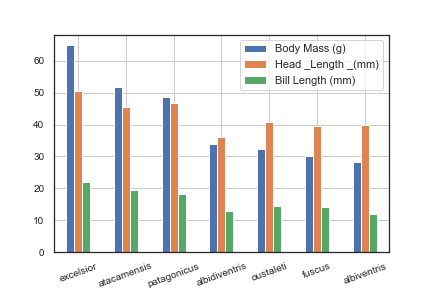
\includegraphics[width=0.9\linewidth]{img/species_ch.png}}
		\caption{\label{depend}Зависимость размеров птиц от вида}
	\end{figure}
Вид \textbf{excelsior} имеет самые внушительные размеры, в то время как вид \textbf{albiventris} проигрывает в этих характеристиках. 
	\subsection{Исследование характеристик в зависимости от страны обитания птиц}
	\begin{figure}[H]
		\center{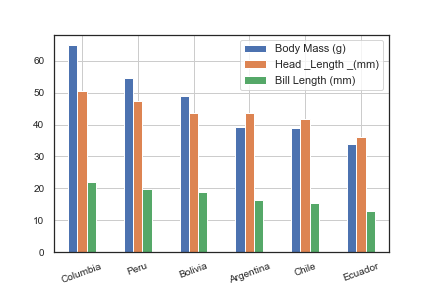
\includegraphics[width=0.9\linewidth]{img/country.png}}
		\caption{\label{depend}Зависимость размеров птиц от страны}
	\end{figure}
В \textbf{Колумбии} можно увидеть самых крупных птиц, а птицы - жители \textbf{Эквадора} достаточно компактны по своим размерам.
\subsection{Корелляция данных}
\begin{figure}[H]
	\center{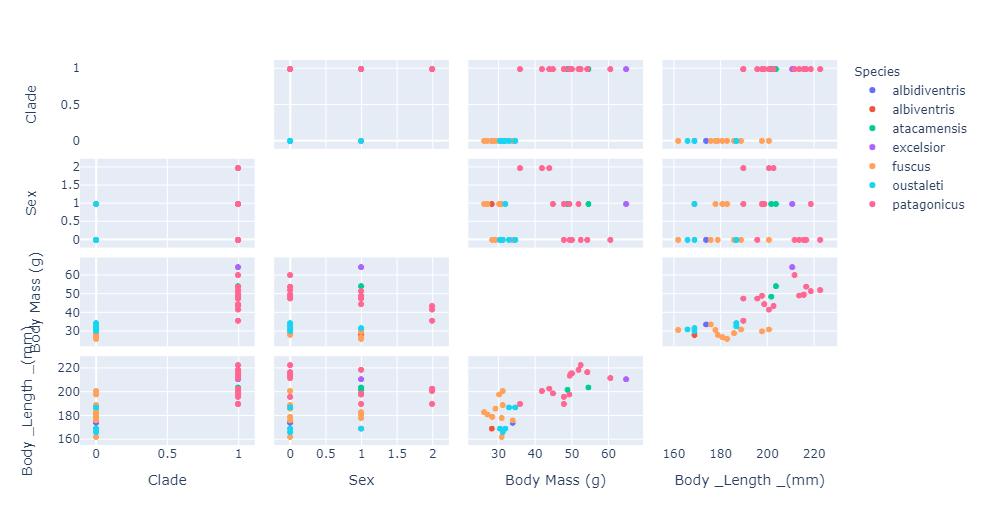
\includegraphics[width=0.9\linewidth]{img/simple.png}}
	\caption{\label{corr}Корреляция выборочных данных}
\end{figure}
\subsection{PCA - метод главных компонент}
При подготовке данных признаки, не имеющие численного представления (строки) были заменены на численное представление, а некоторые удалены. Так же были убраны строки с неизвестным неизвестными параметрами (NaN). В итоге остались 65 признаков и 34 элемента датасета.\\
Дальше данные стандартизировались, для корректной работы метода главных компонент.
\subsubsection{Визуализация основных компонент}
Применён PCA на подготовленный набор данных. 

Пример показывает как количество компонент влияет на разделимость данных. График  PC3 и PC4 явно не может разделить каждый класс, тогда как PC1 и PC2 показывает четкое разделение между каждым видом.

\begin{figure}[H]
	\center{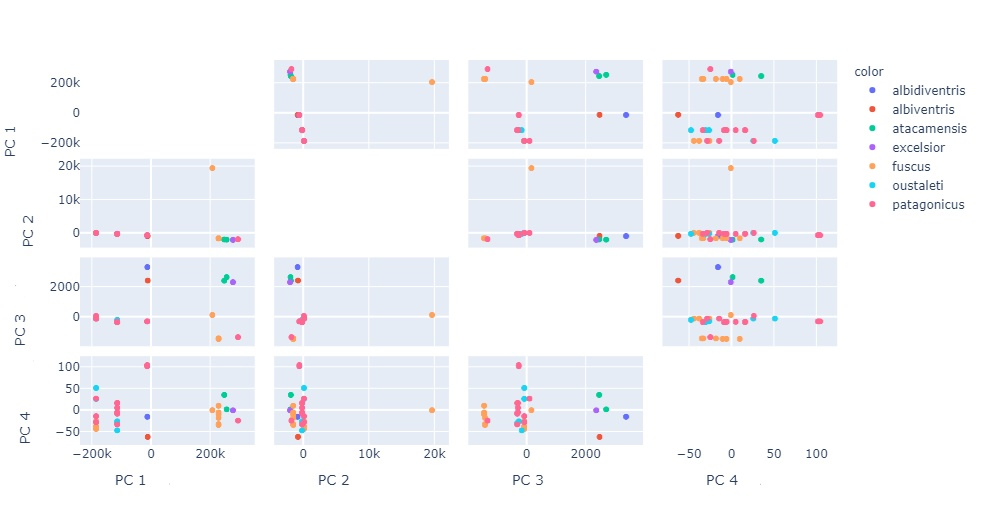
\includegraphics[width=0.9\linewidth]{img/1.jpg}}
	\caption{\label{corr}Корреляция выборочных данных}
\end{figure}
\subsubsection{Зависимость доли общей информации от количества компонент}
\begin{figure}[H]	\center{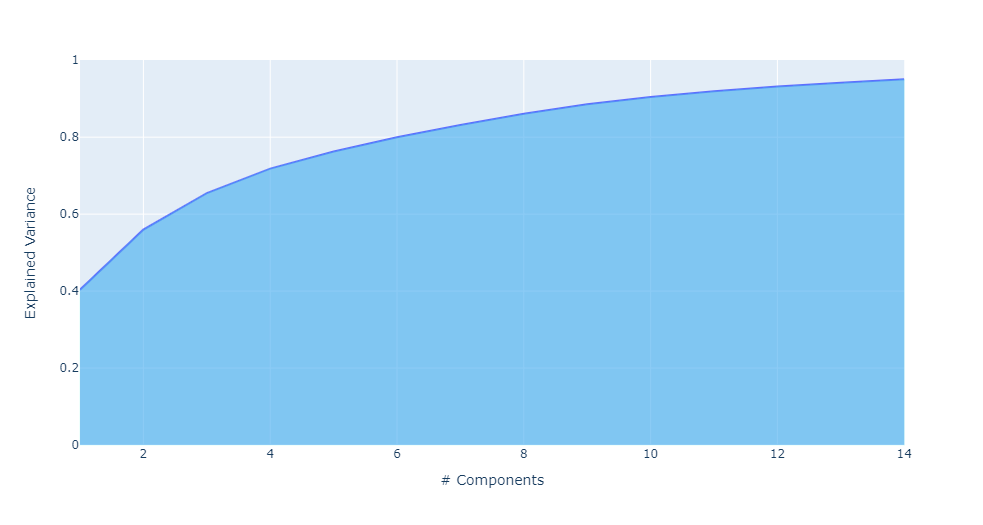
\includegraphics[width=0.9\linewidth]{img/explaned_variance.png}}
	\caption{\label{corr}Корреляция выборочных данных}
\end{figure}	
	\begin{table}[H]
		\centering
		\begin{tabular}{|rrrrrrr|}
			\hline
			1 & 2        & 3        & 4        & 5        & 6        & 7  \\ \hline
			0.416487      & 0.158065 & 0.096908 & 0.061427 & 0.040055 & 0.036198 & 0.032920 \\ \hline
		\end{tabular}
		\centering
		\begin{tabular}{|rrrrrrr|}
			\hline
			8        & 9        & 10      & 11       & 12       & 13       & 14       \\ \hline
			0.026988 & 0.023770 & 0.01928 & 0.014615 & 0.009893 & 0.009483 & 0.007696 \\ \hline
		\end{tabular}
		\caption{\label{tab2}{Доля информация в 14 компонентах}}
	\end{table}
\end{document}